\appendix

\chapter{Amazon Athena } \label{athena-appendix}


\section{Partitionnement de données sur Amazon Athena } \label{subsubsection:partitionnement}~
\subsection{Présentation du partitionnement}
Le partitionnement  de données présentes dans un compartiment Amazon S3 permet de limiter la quantité de données à analyser par une requête Amazon Athena. Le partitionnement améliore  les performances d'Amazon Athena. D'une part, on obtient une réponse rapidement, d'autre part, on réduit les coûts engendrés  suite à l'utilisation du service car on est facturé selon la quantité de données analysées.  

Les partitions créées joue un rôle similaire à celui d'un colonne durant l'interrogation d'une table dans Athena. 

Prenons un exemple, nous avons des traceroutes ayant comme adressage IP la version  4 et d'autres traceroutes ont l'adressage IPv6 :

\begin{lstlisting}
s3://ripeatlasdata/traceroute/
				type=4/
				type=6/
\end{lstlisting}

Sans l'utilisation du partitionnement et si on souhaite récupérer que les traceroutes ayant comme adressage IPv4, toutes les données (type = 4 et type = 6) sont analysées. Toutefois, en partitionnant les données suivant le type d'adressage, seuls les fichiers dans le dossier type = 4 qui sont analysés. Par conséquent, le partitionnement permet de réduire les coûts d'utilisation du service Amazon Athena, surtout si la quantité de données est très importante. 


\subsection{Application du partitionnement sur les traceroutes Atlas}

Les traceroutes en provenance des sondes Atlas sont organisés comme est illustré dans la Figure :

\begin{figure}[H]
	\centering
	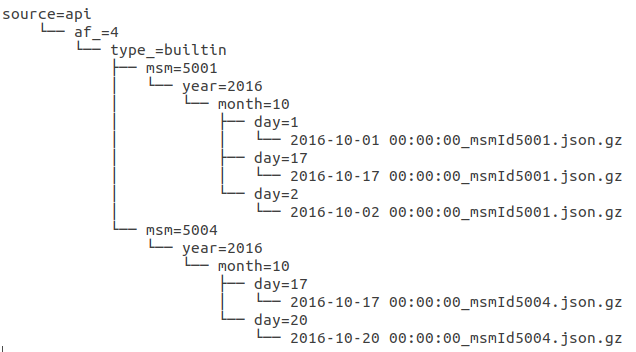
\includegraphics[width=0.6\linewidth]{illustrations/partitionnement-athena}
	\caption{L'organisation des traceroutes dans un compartiment Amazon S3}
	\label{fig:partitionnement-athena}
\end{figure}
 



